\chapter{Fundamentação Teórica}

\section{Lógica na Filosofia e na Matemática}

De início é necessária uma definição de lógica. A lógica ou lógica clássica não foi criada, e sim caracterizada por Aristóteles (384-322 a.C.), podendo ser definida como uma ciência que estuda princípios e métodos de inferência, com o objetivo de determinar em que condições certos fatos são consequência, ou não, de outros \cite{mortari2001}.

Para o filósofo Aristóteles, o objeto da lógica é o silogismo, que é um argumento constituído de proposições das quais se infere uma conclusão, tais proposições devem seguir três princípios fundamentais \cite{zamudio2008tres}: 

\begin{itemize}
    \item \textbf{Princípio da identidade}: Indica a identidade dos seres e das coisas a partir do verbo ser, por exemplo, \textit{"A é A"}.
    \item \textbf{Princípio da não-contradição}: É impossível que um atributo pertença e não pertença ao mesmo sujeito, por exemplo, sabendo que \textit{A é A}, é impossível que \textit{A} seja \textit{não-A}.
    \item \textbf{Princípio do terceiro excluído}: Garante que não haja uma terceira possibilidade, assim duas proposições contraditórias não podem ser ambas verdadeiras em uma mesma relação, por exemplo, (\textit{\{A é x\} e \{A não é x\}}) não é verdade
\end{itemize}

O silogismo em si, trata-se de uma estrutura linguística dedutiva, baseada na existência de duas premissas e uma conclusão tirada a partir das mesmas, como demonstra o exemplo a seguir \cite{mortari2001}:

\begin{quote}\centering
    \textit{Todo gato é mamífero \\
    Miau é um gato \\
    Miau é mamífero}
\end{quote}

Essa sequência de premissas e uma conclusão é o primeiro passo para a lógica proposicional, que trata de interpretar enunciados atribuindo valores verdade às suas proposições, podendo incluir operações que permitem construir proposições complexas, como as operações de conjunção ("E"), disjunção ("OU"), implicação ("SE ... ENTÃO ...") e negação ("NÃO") \cite{flavio2010}. A tabela \ref{tab:log}, demonstra uma comparação entre a lógica clássica e a lógica proposicional, indicando um dos operadores proposicionais, o "ENTÃO".

\begin{table}[!htb]
\centering
	\caption[Comparação entre a lógica clássica no mundo real e a lógica proposicional]{Comparação entre a lógica clássica no mundo real e a lógica proposicional}
	\label{tab:log}
\begin{tabular}{c|c}
\hline \SPACE
\textbf{MUNDO REAL}                             & \textbf{PROPOSIÇÃO LÓGICA} \\ \hline \SPACE
Hoje está chovendo                              & $P$                          \\ \hline \SPACE
A rua está molhada                              & $Q$                          \\ \hline \SPACE
Se hoje está chovendo, então a rua está molhada & $P \rightarrow Q$          \\ \hline
\end{tabular}
\fonte{Próprio Autor.}
\end{table}

A lógica matemática nasce a partir da lógica proposicional em meados do século XIX, pelos tratamentos matemáticos sistemáticos de George Boole (1815 - 1864) e Augustus De Morgan (1806 - 1871), que nos permite interpretar proposições matemáticas de forma a julgá-las como verdadeiras ou falsas \cite{ferreiros2001}. Com a lógica matemática pode-se representar os operadores proposicionais em operadores lógicos para a formulação de afirmações matemáticas.


\section{Lógica de Ordem Zero e Lógica de Primeira Ordem}

A lógica proposicional contém um conjunto de fórmulas, que pode ser denominado como \simbolo{$L_\emptyset$}{Lógica de ordem zero}, também conhecido como lógica de ordem \simbolo{$\emptyset$}{Vazio}, bem como existe uma extensão da lógica proposicional que é chamada de Lógica de Primeira Ordem (\sigla{LPO}{Lógica de Primeira Ordem}). A principal diferença entre as duas é basicamente o que cada linguagem pressupõe sobre a natureza da realidade. Enquanto a $L_\emptyset$ assume que existem fatos verdadeiros ou falsos no mundo, a LPO pressupõe que as relações entre determinados objetos são válidas ou não-válidas \cite{fonseca2012logica}.

Esta seção apresenta um estudo da $L_\emptyset$ e da LPO dividindo ambos em suas abordagens semântica e sintática.

\subsection{Sintaxe da Lógica de Ordem Zero}

O primeiro passo para compreender a $L_\emptyset$, é entender os seus conectivos, sabendo que cada formula é uma proposição gerada pela concatenação de símbolos pertencentes ao alfabeto da $L_\emptyset$ que é composto pelos seguintes itens:

\begin{itemize}
    \item \textbf{Símbolos proposicionais}: $\wp = \{P, Q, R, S, P_1, P_2, ...\}$
    \item \textbf{Conectivos}: Unários e binários, demonstrados na tabela \ref{tab:cp}
    \item \textbf{Elementos de pontuação}: '(' e ')'
\end{itemize}

\begin{table}[!htb]
\centering
	\caption[Conectivos proposicionais]{Conectivos proposicionais}
	\label{tab:cp}
\begin{tabular}{c|c}
\hline \SPACE
\textbf{CONECTIVO} & \textbf{SIGNIFICADO} \\ \hline \SPACE
\simbolo{$\neg$}{Negação lógica (NÃO)}                  & "NÃO"                \\ \hline \SPACE
\simbolo{$\lor$}{Disjunção lógica (OU)}                  & "OU"                 \\ \hline \SPACE
\simbolo{$\land$}{Conjunção lógica (E)}                  & "E"                  \\ \hline \SPACE
\simbolo{$\rightarrow$}{Implicação lógica (SE...ENTÃO)}                  & "SE ... ENTÃO ..."   \\ \hline \SPACE
\simbolo{$\leftrightarrow$}{Bicondicional lógica (SE E SOMENTE SE)}                  & "SE E SOMENTE SE"    \\ \hline
\end{tabular}
\fonte{\cite{flavio2010}}
\end{table}

Assim como na língua portuguesa, na $L_\emptyset$ nem toda concatenação é válida. Os elementos da $L_\emptyset$ são chamados de fórmulas, sendo que cada formula segue um conjunto de regras para sua formação \cite{mendelson2009introduction}: 

\begin{enumerate}
    \item Todos os símbolos proposicionais são chamados de fórmulas
    \item Se $P$ é uma fórmula, então $\neg P$ também é uma fórmula
    \item Se $P$ e $Q$ são fórmulas, então ($P \lor Q$), ($P \land Q$), ($P \rightarrow Q$) e ($P \leftrightarrow Q$) também são fórmulas
\end{enumerate}

O conectivo $\neg$ também se aplica a todas as regras acima. Utilizando as mesmas de forma recursiva, com a aplicação dos parênteses quando necessário, é possível obter um conjunto infinito de fórmulas.

\subsection{Semântica da Lógica de Ordem Zero}

A semântica da $L_\emptyset$ consiste basicamente em atribuir valores verdade (verdadeiro ou falso) às fórmulas da linguagem, com o objetivo de saber se seu resultado é verdadeiro ou falso. Para realizar essa validação existem diversos métodos de inferência, tais como, tabelas-verdade, tablôs semânticos, princípio da resolução e dedução natural \cite{flavio2010}.

\subsubsection{Tabela-Verdade}

O método da tabela-verdade tem o objetivo de determinar a validade de um argumento atribuindo valores verdadeiros ou falsos para todos os símbolos proposicionais, examinando todos os casos possíveis e gerando uma visão geral de toda a fórmula, sendo que para um conjunto infinito de letras sentenciais tem-se um conjunto também infinito de valorações \cite{mortari2001}, onde cada um dos operadores lógicos gera um determinado resultado, como demonstrado na tabela \ref{tab:basic-values}.

\begin{table}[!htb]
\centering
\caption[Tabela-verdade básica]{Tabela-verdade básica}
\label{tab:basic-values}
\begin{tabular}{c|c|c|c|c|c|c|c}
\hline
\textbf{P} & \textbf{Q} & \textbf{$\neg$P} & \textbf{$\neg$Q} & \textbf{$\mathbf{P \lor Q}$} & \textbf{$\mathbf{P \land Q}$} & \textbf{$\mathbf{P \rightarrow Q}$} & \textbf{$\mathbf{P \leftrightarrow Q}$} \\ \hline
V          & V          & F                & F                & V            & V                             & V                          & V                                     \\ \hline
V          & F          & F                & V                & V            & F                             & F                          & F                                     \\ \hline
F          & V          & V                & F                & V            & F                             & V                          & F                                     \\ \hline
V          & F          & V                & V                & F            & F                             & V                          & V                                     \\ \hline
\end{tabular}
\fonte{\cite{mortari2001}}
\end{table}

Um exemplo de tabela-verdade simples pode ser dado a partir da fórmula $(\neg A \land \neg B) \rightarrow \neg A $, atribuindo valores verdade para A e/ou B. Partindo desses valores pode-se construir a tabela \ref{tab:tva}.

\begin{table}[!htb]
\centering
\caption[Tabela-verdade para a expressão $\mathbf{(\neg A \land \neg B) \rightarrow \neg A }$]{Tabela-verdade para a expressão $\mathbf{(\neg A \land \neg B) \rightarrow \neg A }$}
\label{tab:tva}
\begin{tabular}{c|c|c|c|c}
\hline
\textbf{A} & \textbf{B} & $\mathbf{\neg A}$ & $\mathbf{\neg A \land \neg B}$ & $\mathbf{(\neg A \land \neg B) \rightarrow \neg A}$ \\ \hline
V          & V          & F          & F          & V          \\ \hline
F          & V          & V          & V          & V          \\ \hline
V          & F          & F          & F          & V          \\ \hline
F          & F          & V          & F          & V          \\ \hline
\end{tabular}
\fonte{\cite{mortari2001}}
\end{table}

Quando se tem uma fórmula onde todas as suas valorações são verdadeiras, a mesma é denominada tautologia.

\subsection{Sintaxe da Lógica de Primeira Ordem}

\subsubsection{Símbolos}

A LPO faz a suposição de que o mundo é constituído de objetos com certas propriedades ou relações entre eles, onde os objetos podem ser definidos em função de outros objetos e suas relações podem ser verdadeiras ou falsas. A linguagem geral do cálculo de predicados de primeira ordem é formada por símbolos lógicos e não-lógicos \cite{mortari2001}, que devidamente agrupados formam os axiomas. 

\begin{itemize}
    \item \textbf{Símbolos lógicos}: 
        \begin{itemize}
            \item \textit{Símbolos de constantes}: um conjunto enumerável de nomes específicos de objetos no domínio do discurso.
            \item \textit{Símbolos de predicados}: um conjunto enumerável de símbolos que representam relações.
        \end{itemize}
        Ambos são representados por letras maiúsculas (\textit{A, B, X, Y}, etc)
        
    \item \textbf{Símbolos não-lógicos}:
        \begin{itemize}
            \item \textit{Variáveis}: Nomeiam um conjunto de objetos, geralmente representadas por letras minúsculas (\textit{x}, \textit{y}, \textit{z}, etc).
            \item \textit{Operadores}: Incluem os conectivos unários e binários demonstrados na tabela \ref{tab:cp}.
            \item \textit{Quantificadores}: O quantificador universal $\forall$ e o quantificador existencial $\exists$.
            \item \textit{Sinais de pontuação}:  '(' e ')'.
        \end{itemize}
\end{itemize}

\subsubsection{Fórmulas}

A partir do conjunto acima de símbolos, podem ser construídas as fórmulas que definem a composição de uma proposição, por exemplo, considerando a afirmação "x é um filósofo", é possível escolher um símbolo de predicado para representar o fato de ser um filósofo, podendo ser F por exemplo. Em seguida infere-se que x pode ser qualquer indivíduo, esse é uma variável, podendo ser 'a':

\begin{itemize}
    \item \textit{F}: 'x é um filósofo'
    \item \textit{a}: Aristóteles
\end{itemize}

A partir dos dados acima é possível construir uma fórmula que representa que "Aristóteles é um filósofo" usando a notação '\textit{Fa}', essa é a formula mais simples que se tem na LPO, sendo denominada fórmula atômica \cite{mortari2001}. Não existe uma convenção que defina a ordem de construção de uma fórmula atômica, porém é necessário que se mantenha uma homogeneidade na construção das fórmulas. Adicionando mais variáveis, é possível construir sentenças mais complexas usando somente fórmulas atômicas, se for acrescentado que Platão também é um filósofo, representando o mesmo pela letra '\textit{p}', a fórmula \textit{Fpa} representa que Platão e Aristóteles são filósofos.

Caso uma sentença tenha mais de uma fórmula atômica, a mesma é denominada de fórmula molecular, nesse caso entra o uso dos conectivos (tabela \ref{tab:cp}) para realizar a composição de uma fórmula. Tomando como base a fórmula \textit{Fpa} citada anteriormente, pode-se adicionar mais uma fórmula atômica, por exemplo:

\begin{itemize}
    \item \textit{M}: 'x é um matemático'
    \item \textit{f}: Fourier
\end{itemize}

Assim pode-se construir a fórmula molecular que infere que Platão e Aristóteles são filósofos e Fourier é matemático, da seguinte maneira, sendo os parênteses facultativos nesse caso:

\begin{quote}\centering
    (\textit{Fpa} $\land$ \textit{Mf})
\end{quote}

Como afirmado por \citeonline{mendelson2009introduction}, citado anteriormente na seção 2.2.1, usando os conectivos proposicionais podem se formar diversas fórmulas onde \textit{P} e \textit{Q} podem ser tanto fórmulas atômicas quanto moleculares.

Segundo \citeonline{mortari2001}, Uma linguagem de primeira ordem é qualquer subconjunto da linguagem geral do cálculo de predicados de primeira ordem (\sigla{CQC}{Cálculo Quantificacional Clássico de Primeira Ordem}) que inclua todos os símbolos lógicos e pelo menos uma constante de predicado. Essa informação infere que é possível construir fórmulas se dispuser de pelo menos um símbolo de predicado.

Para fórmulas moleculares um pouco mais complexas, pode-se usar parênteses como auxiliares, como no exemplo dado por \citeonline{mortari2001}, "Salma Hayek é morena, mas Claudia Schiffer e Cameron Díaz não o são". Essa expressão pode ser agrupada com colchetes e reescrita com outras palavras para facilitar o seu entendimento, como [Salma Hayek é morena] mas [Claudia Schiffer não é morena e Cameron Díaz não é morena]. Considerando M como "x não é morena", os indivíduos como \textit{s}, \textit{c} e \textit{d} respectivamente, usando os parênteses de maneira correta obtém-se a fórmula $(Ms \land (\neg Mc \land \neg Md))$.

Para fórmulas ainda mais complexas, pode-se usar os quantificadores universal (\simbolo{$\forall$}{Para todo}) e existencial (\simbolo{$\exists$}{Existe}), como no exemplo dado por \citeonline{mendelson2009introduction}, \textit{"Qualquer amigo de Martin é amigo de John"}, usando o quantificador universal, considerando as varáveis \textit{m} e \textit{j} para os indivíduos respectivamente e F como "x é amigo", é construída a fórmula $\forall x (Fxm \rightarrow Fxj)$. Da mesma forma pode-se elaborar um exemplo com o quantificador existencial, como \textit{"Algumas pessoas são amigas de Martin e John"}, formulado como: $\exists x (Fxm \land Fxj)$.

\subsubsection{Formas básicas de proposição categórica}

De forma geral, várias sentenças de estrutura mais complexa podem ser reduzidas às formas básicas de proposição categórica (tabela \ref{tab:basic}), porém há muitos exemplos que não se encaixam nesse padrão e devem ser cuidadosamente analisados para um correto resultado \cite{mortari2001}.

\begin{table}[!htb]
\centering
	\caption[Formas básicas de proposição categórica]{Formas básicas de proposição categórica}
	\label{tab:basic}
\begin{tabular}{c|c}
\hline \SPACE
Todo A é B                  & $\forall x (Ax \rightarrow Bx)$                \\ \hline \SPACE
Nenhum A é B                & $\forall x (Ax \rightarrow \neg Bx)$                 \\ \hline \SPACE
Algum A é B                  & $\exists x (Ax \land Bx)$                  \\ \hline \SPACE
Algum A não é B                  & $\exists x (Ax \land \neg Bx)$   \\ \hline
\end{tabular}
\fonte{\cite{mortari2001}}
\end{table}

\subsection{Semântica da Lógica de Primeira Ordem}

De maneira análoga a $L_\emptyset$, para a LPO o estudo da semântica é feito realizando a atribuição de valores verdade onde tais valores são destinados às sentenças moleculares, para então realizar a interpretação desses valores na fórmula geral, definindo suas relações. Isso permite a definição de consequência lógica (\simbolo{$\models$}{Consequência lógica}), denotado por $\Gamma \models \alpha$, cujo significado segundo \citeonline{mortari2001} é que se $\Gamma$ é um conjunto de fórmulas, e \simbolo{$\alpha$}{Letra grega Alfa} uma fórmula, dizemos que $\alpha$ é uma consequência lógica de \simbolo{$\Gamma$}{Letra grega Gama} se e somente se todo modelo de $\Gamma$ é também modelo de $\alpha$. Em outras palavras, segundo \citeonline{Tannen2009}, a sentença $\alpha$ é verdadeira em qualquer estrutura na qual as sentenças do conjunto $\Gamma$ são verdadeiras.

\subsubsection{Validade e tabelas-verdade}

As fórmulas podem ser classificadas em três tipos:

\begin{itemize}
    \item \textbf{Tautológicas}: Verdadeiras em todas as valorações.
    \item \textbf{Contradições}: Falsas em todas as valorações.
    \item \textbf{Contingências}: Verdadeiras em ao menos uma e falsas em ao menos uma valoração.
\end{itemize}

A partir do conceito de tautologia, pode-se definir um novo conceito para a LPO, o de fórmula válida, que denota uma fórmula verdadeira em toda e qualquer estrutura \cite{mortari2001}. Tautologias funcionam de maneira eficaz na $L_\emptyset$, porém na LPO verifica-se que nem todas as fórmulas válidas são tautologias. 

Tomando o seguinte exemplo com duas fórmulas elementares: $\forall xPx \rightarrow Pa$, apesar de ser uma fórmula válida, na tabela \ref{tab:tautologia}, vemos que ela não é uma tautologia, isso acontece porque tabelas-verdade não conseguem lidar bem com quantificadores, pois numa fórmula como $\forall xPx$ por exemplo, é impossível obter o seu valor, visto que tem um universo infinito de casos possíveis. Com isso existem outros métodos eficazes de mostrar a validade de uma estrutura na LPO, alguns deles serão citados a seguir.

\begin{table}[!htb]
\centering
	\caption[Tabela-verdade para uma fórmula válida]{Tabela-verdade para uma fórmula válida}
	\label{tab:tautologia}
\begin{tabular}{c|c|c}
\hline \SPACE
\textbf{$\forall xPx$} & \textbf{$Pa$} & \textbf{$\forall xPx \rightarrow Pa$} \\ \hline \SPACE
V                  & V        &   V     \\ \hline \SPACE
F                  & V           &  V    \\ \hline \SPACE
V                  & F            &   F   \\ \hline \SPACE
F                  & F  &  V \\ \hline
\end{tabular}
\fonte{\cite{mortari2001}}
\end{table}

\subsection{Tablôs Semânticos}

Também conhecido como árvores de refutação, o método de inferência por tablôs semânticos permite mostrar a validade ou invalidade de um fórmula, ou determinar se alguma fórmula é consequência lógica, ou não, de algum conjunto de fórmulas usando um procedimento de prova \cite{mortari2001}. Esse é um dos métodos ideais para lidar com a lógica de primeira ordem, pois consegue realizar validações com base nos quantificadores universal e existencial. 

Tomando como exemplo a fórmula $\forall xPx \rightarrow Pa$ citada anteriormente, pode-se interpreta-la como: se é verdade que todos são matemáticos, então é verdade que Fourier é matemático. Mesmo sabendo que é uma expressão verdadeira, o passo inicial é assumir que a expressão é falsa na primeira linha do tablô, e seguir os passos de comparação com o auxílio da tabela \ref{tab:basic-values}:

\begin{quote}\centering
    $\checkmark$ \textbf{F} $\forall xPx \rightarrow Pa$ \\
    \textbf{V} $\forall xPx$ \\
    \textbf{F} $Pa$
\end{quote}

Partindo para a segunda fórmula, pode-se concluir que se todos são matemáticos então $Pa$, $Pb$, $Pc$ e os demais são matemáticos, logo $Pa$ é verdadeiro, finalizando o tablô da seguinte maneira: 

\begin{quote}\centering
    $\checkmark$ \textbf{F} $\forall xPx \rightarrow Pa$ \\
    \textbf{V} $\forall xPx$ \\
    \textbf{F} $Pa$ \\
    \textbf{V} $Pa$ \\
    X
\end{quote}

\subsection{Dedução Natural}

A Dedução Natural é um sistema de prova que permite extrair conclusões a partir de um conjunto de premissas, que são fórmulas de uma lógica construídas de acordo com as regras de formação da linguagem. Isso nos permite inferir fórmulas a partir de outras fórmulas, por meio de regras denominadas regras de inferência. Ao aplicar essas regras em sucessão, podemos tirar uma conclusão a partir de um conjunto de premissas, que pode servir como premissa na obtenção de novas conclusões e assim sucessivamente \cite{huth2004logic}.

Uma dedução é construída inicialmente listando as premissas que estão ao nosso dispor e uma outra fórmula chamada de conclusão, que é o objetivo a ser atingido. Após isso podem ser aplicadas regras de inferência que permitem acrescentar uma nova linha à essa lista, contendo uma fórmula que é o resultado da aplicação da regra às fórmulas anteriores \cite{mortari2001}. Ao aplicar as regras de inferência a essas fórmulas, pode-se eventualmente obter a conclusão. Tomando \simbolo{$\phi$}{Letra graga Phi} como a lista de fórmulas e \simbolo{$\psi$}{Letra grega Psi} como a fórmula de conclusão, isso pode ser denotado por:

\begin{quote}\centering
    $\phi_1, \phi_2, ..., \phi_n \models \psi $
\end{quote}

\subsubsection{Regras de inferência diretas}

São as regras que regulam quais fórmulas podem ser inferidas a partir de outras fórmulas (figura \ref{fig:diretas}).

\begin{figure}[!htb]
	\centering
	\caption[Regras de inferência diretas]{Regras de inferência diretas.}
	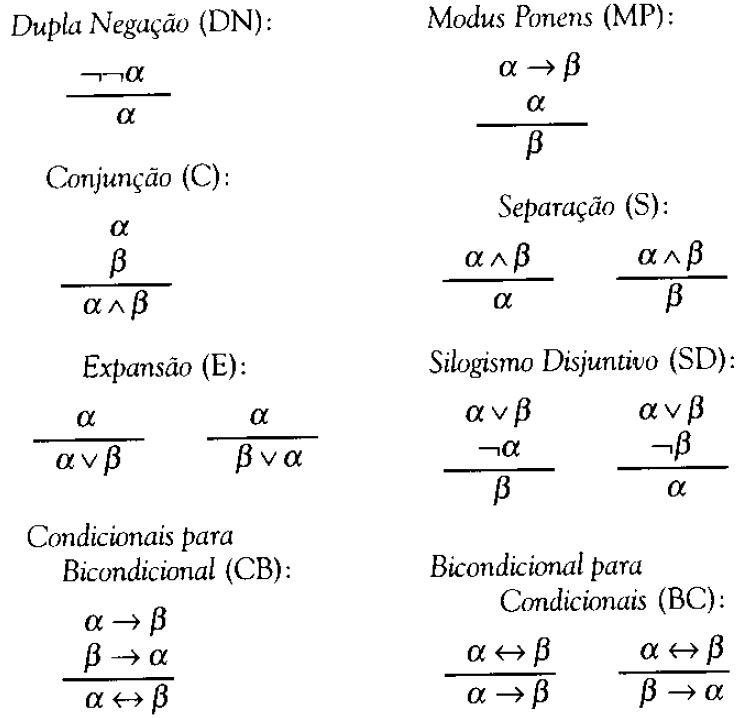
\includegraphics[width=0.6\textwidth]{diretas.png}
	\fonte{MORTARI, 2001\nocite{mortari2001}}
	\label{fig:diretas}
\end{figure}

\subsubsection{Regras de inferência hipotéticas}

Exigem o uso de hipóteses, usadas para os operadores não citados nas regras diretas, são as regras de redução ao absurdo e regra de prova condicional (figura \ref{fig:hip}). Na regra de redução ao absurdo (\sigla{RAA}{Regra de redução ao absurdo}), a partir de uma hipótese $\alpha$, deriva-se uma contradição $\beta \land \neg \beta$, então pode-se descartar $\alpha$ e introduzir $\neg \alpha$ na derivação. Na regra de prova condicional (\sigla{RPC}{Regra de prova condicional}), a partir de uma hipótese $\alpha$ que deriva uma fórmula \simbolo{$\beta$}{Letra grega Beta}, pode-se descartar $\alpha$ e introduzir $\alpha \rightarrow \beta$ na derivação \cite{mortari2001}.

\begin{figure}[!htb]
	\centering
	\caption[Regras de inferência hipotéticas]{Regras de redução ao absurdo e regra de prova condicional, respectivamente.}
	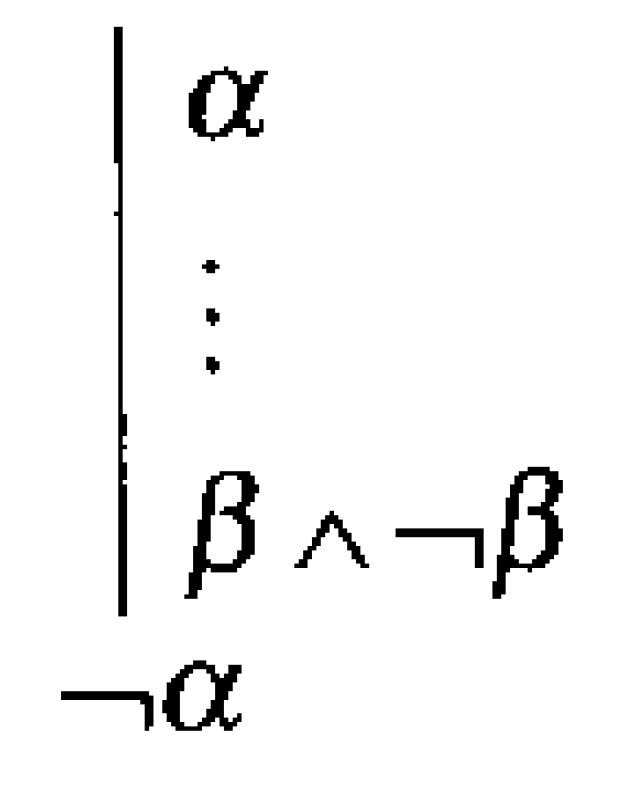
\includegraphics[width=0.15\textwidth]{raa.png}
	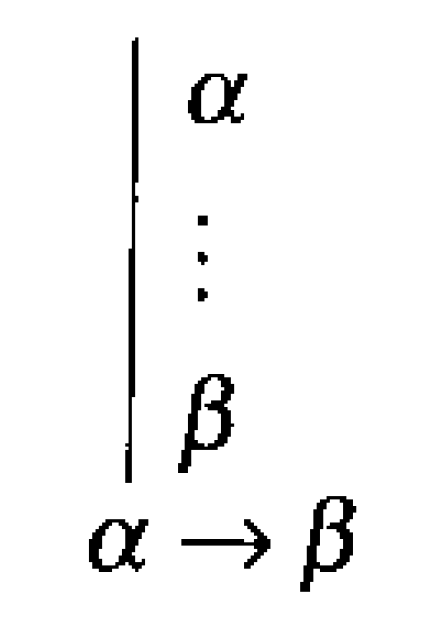
\includegraphics[width=0.15\textwidth]{rpc.png}
	\fonte{MORTARI, 2001\nocite{mortari2001}}
	\label{fig:hip}
\end{figure}

\subsubsection{Regras de inferência derivadas}

Podem ser provadas a partir das outras regras, de modo que tudo que pode ser feito com uma regra derivada, também pode ser feito usando as regras iniciais, mostrando que uma regra derivada é uma maneira de abreviar parte de uma dedução, facilitando o procedimento. a figura \ref{fig:derivadas} demonstra algumas dessas regras.

\begin{figure}[!htb]
	\centering
	\caption[Algumas regras de inferência derivadas]{Algumas regras de inferência derivadas.}
	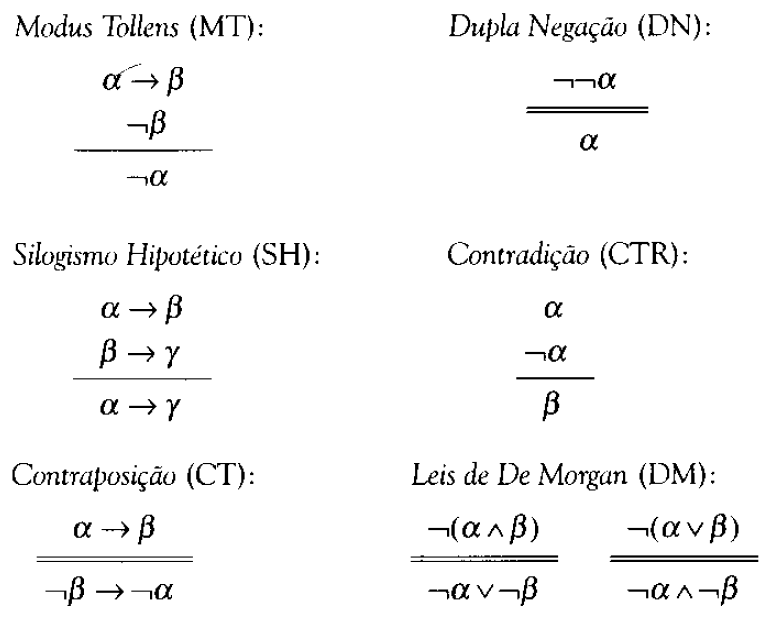
\includegraphics[width=0.6\textwidth]{derivadas.png}
	\fonte{MORTARI, 2001\nocite{mortari2001}}
	\label{fig:derivadas}
\end{figure}

\subsubsection{Regras para quantificadores}

Completam todo o conjunto de regras da dedução natural, e são usadas para lidar com os quantificadores universal e existencial, são quatro regras, sendo elas as regras de eliminação e introdução dos quantificadores universal (figura \ref{fig:universal}) e existencial (figura \ref{fig:existencial}).

\begin{figure}[!htb]
	\centering
	\caption[Regras para o quantificador universal]{Regras para o quantificador universal.}
	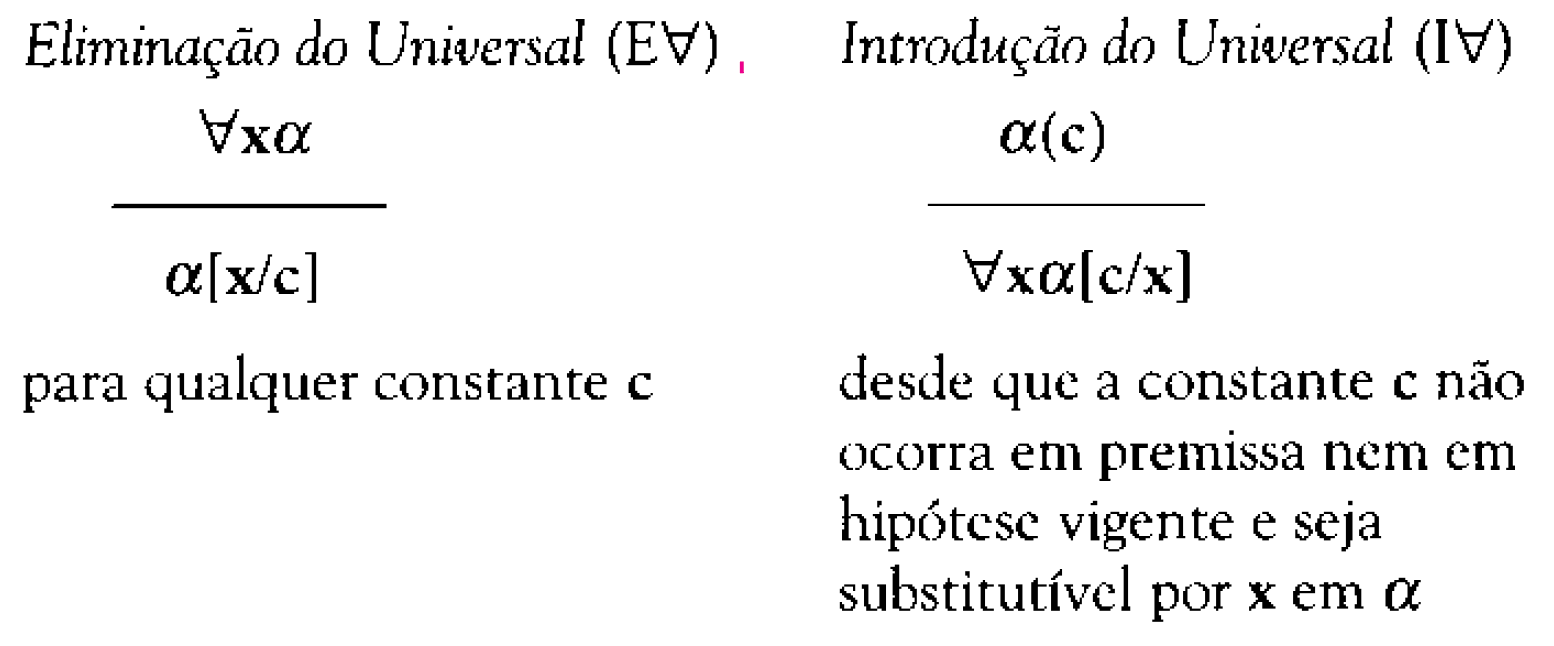
\includegraphics[width=0.6\textwidth]{universal.png}
	\fonte{MORTARI, 2001\nocite{mortari2001}}
	\label{fig:universal}
\end{figure}

\begin{figure}[!htb]
	\centering
	\caption[Regras para o quantificador existencial]{Regras para o quantificador existencial.}
	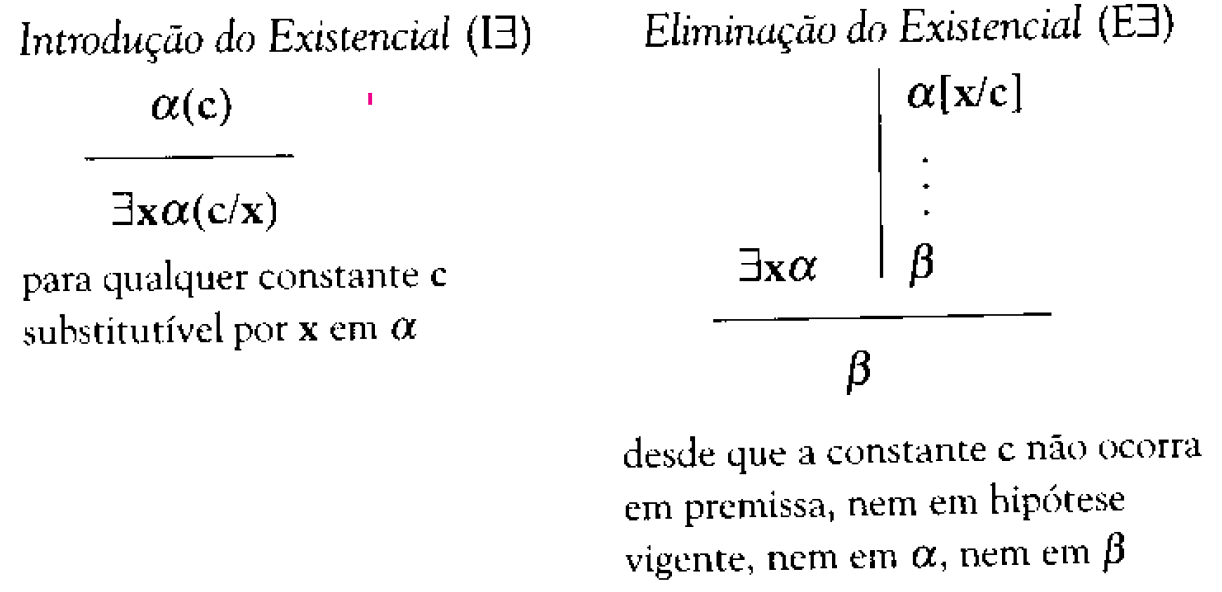
\includegraphics[width=0.6\textwidth]{existencial.png}
	\fonte{MORTARI, 2001\nocite{mortari2001}}
	\label{fig:existencial}
\end{figure}

\section{Problema da Satisfatibilidade Booleana}

O problema da satisfatibilidade booleana (SAT) trata da verificação da existência de uma atribuição de valores verdadeiro ou falso que torne em verdadeira uma fórmula booleana expressa em forma normal conjuntiva (\sigla{FNC}{Forma Normal Conjuntiva}). Esse problema ocupa um papel fundamental na ciência da computação teórica, especialmente no contexto da teoria de complexidade de problemas. Diante de uma fórmula booleana, o desafio é determinar se há uma combinação de valores para suas variáveis que faça com que a expressão seja satisfeita \cite{el2016computational}.

O SAT foi o primeiro problema a ser demonstrado como NP-completo \cite{cook2023complexity}, ou seja, qualquer problema em \sigla{NP}{Tempo polinomial não determinístico} pode ser reduzido a SAT em tempo polinomial: para todo problema \( L \) em NP, existe uma função computável polinomialmente que, dada uma instância \( w \) de \( L \), constrói uma fórmula em FNC satisfazível se, e somente se, \( w \in L \). A prova técnica envolve codificar o funcionamento de uma máquina de \textit{Turing} não determinística na estrutura lógica da fórmula, de modo que satisfazer a fórmula equivale a simular a aceitação da máquina \cite{Cook_Levin-AFP}. Toda a importância solução do SAT, alavancou o desenvolvimento de algoritmos otimizados para resolve-lo, se tornando um objetivo crucial na área de pesquisa em algoritmos e complexidade. 

Na prática, apesar de sua complexidade, muitos exemplos do SAT são tratáveis por \textit{solvers} contemporâneos, que combinam algoritmos como \sigla{DPLL}{Davis–Putnam–Logemann–Loveland} (Davis–Putnam–Logemann–Loveland), \sigla{CDCL}{Conflict‑Driven Clause Learning} (Conflict‑Driven Clause Learning) e busca local. Além disso, há pesquisas recentes aplicando técnicas de aprendizado de máquina para melhorar heurísticas \textit{solver} \cite{guo2023machine}.

\subsection{O Problema MAX-SAT}

O MAX-SAT é uma extensão do clássico problema de SAT, onde o objetivo não é apenas encontrar uma atribuição que satisfaça todas as cláusulas de uma fórmula na FNC, mas sim a que maximiza o número de cláusulas satisfeitas, caracterizando o seu nome em tradução livre para o português como Satisfatibiliade Máxima. Formalmente, dada uma fórmula \( \varphi = C_1 \land C_2 \land \cdots \land C_k \) composta por cláusulas \( C_i \), busca-se uma atribuição \textit{booleana} \( A \) que maximize a quantidade de cláusulas para as quais \( A(C_i) = \textit{true} \) \cite{el2016computational}. 

Considerando que a quantidade de cláusulas tem no máximo 2 literais cada, temos a versão restrita conhecida como MAX‑2‑SAT e assim sucessivamente para \textit{n} literais. Apesar dessa simplificação estrutural, essa variante continua NP-completa na versão de decisão (isto é, determinar se existe uma atribuição que satisfaça pelo menos \textit{k} cláusulas). A formulação geral do MAX‑SAT também pertence à classe NP-completo, conforme demonstrado em estudos clássicos de complexidade \cite{krentel1986complexity}.

Esse problema é fundamental tanto teoricamente quanto na prática. Ele aparece em domínios como, verificação de hardware e software, roteamento de satélites, \textit{timetabling}, entre outros tópicos da Ciência da Computação e Engenharia Elétrica. Consequentemente, há intenso esforço acadêmico voltado a \textit{solvers} que sejam capazes de resolver grandes conjuntos de exemplos do MAX-SAT, bem como a heurísticas e algoritmos aproximados \cite{biere2009handbook}. 

\subsection{Transição de Fase}

A transição de fase em problemas SAT é um fenômeno observado quando se estuda o comportamento de instâncias aleatórias de fórmulas booleanas em função da razão entre cláusulas e variáveis. Especificamente, à medida que aumentamos essa razão, existe um ponto crítico no qual a probabilidade de que uma fórmula seja satisfatível cai abruptamente de quase 1 para quase 0, esse ponto é conhecido como limiar de transição de fase e tem sido intensamente estudado por sua relevância teórica e prática em ciência da computação, especialmente na análise de desempenho de algoritmos de resolução de SAT \cite{cheeseman1991really}. 

Estudos realizados por \citeonline{mitchell1992hard} observaram que instâncias de problemas SAT aleatórios são mais difíceis de resolver quando a razão entre o número de cláusulas e o número de variáveis se aproxima de um valor crítico. Abaixo desse valor, a maioria das instâncias é satisfazível e fácil de resolver, enquanto acima dele, a maioria é insatisfazível e também relativamente fácil de provar sua insatisfatibilidade.

Um estudo realizado por \citeonline{crawford1996experimental}, demonstrou graficamente a relação entre a porcentagem de satisfatibilidade e a dificuldade de um problema \textit{3-SAT} para 200 variáveis aleatórias, considerando a razão $\alpha$ de cláusula/variável. A figura \ref{fig:phase-graph} exemplifica o ponto de transição de fase graficamente, onde uma linha mostra a porcentagem satisfazível e a outra mostra a dificuldade do problema. A dificuldade do problema atinge o pico na região onde a porcentagem satisfazível cai repentinamente de quase cem por cento para quase zero. À medida que $\alpha$ aumentava de 0 para 4,3, o problema começava fácil, exigindo um pequeno número de lançamentos para encontrar uma solução, para difícil, exigindo significativamente mais lançamentos, e então para fácil novamente após $\alpha$ = 4,3 \cite{qasem2009sat}.

\begin{figure}[!htb]
	\centering
	\caption[Demonstração do ponto de transição de fase]{Demonstração do ponto de transição de fase.}
	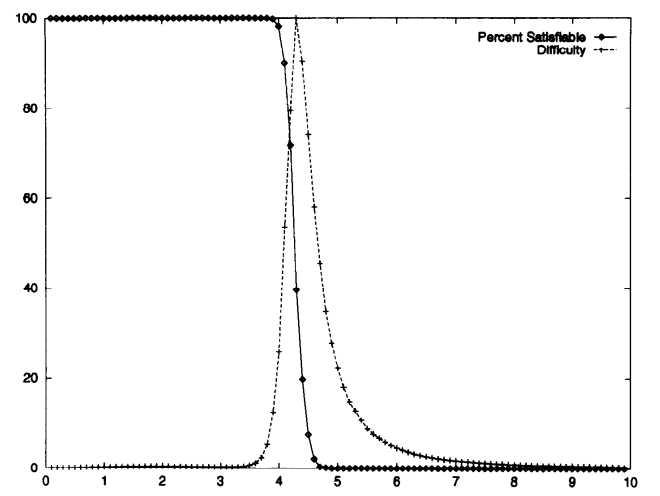
\includegraphics[width=0.6\textwidth]{phase-graph.png}
	\fonte{CRAWFORD; AUTON, 1996\nocite{crawford1996experimental}}
	\label{fig:phase-graph}
\end{figure}

No contexto do MAX-SAT a transição de fase também se manifesta, embora de forma mais complexa. Em vez de um comportamento binário, o foco está na fração de cláusulas que podem ser satisfeitas à medida que a razão $\alpha$ varia. Estudos como os de \citeonline{monasson1999determining} mostraram que existe uma mudança abrupta no comportamento estatístico dessas instâncias, especialmente no número esperado de cláusulas satisfeitas e na estrutura das soluções. Essa mudança tem implicações diretas na tratabilidade dos problemas, onde quando próximos à transição de fase, instâncias tendem a ser mais difíceis de resolver, demandando mais tempo computacional, tanto por algoritmos exatos quanto por heurísticas.

Compreender a transição de fase no MAX-SAT é essencial para o desenho de algoritmos mais eficientes e para a análise de complexidade média. O estudo desses fenômenos indica que as regiões de transição carregam informações cruciais sobre a estrutura do espaço de soluções e o comportamento típico de instâncias difíceis, abrindo caminho para avanços tanto teóricos quanto práticos na computação.
 
\subsection{SAT Solvers}

\textit{SAT solvers} são ferramentas computacionais desenvolvidas para solucionar problemas SAT, e tornaram-se essenciais em áreas como verificação formal, inteligência artificial e otimização. \textit{Solvers} para MAX-SAT adaptam técnicas dos \textit{SAT Solvers}, incorporando estratégias específicas para balancear eficiência e qualidade da solução, esses \textit{solvers} buscam encontrar a atribuição de variáveis que maximiza o número de cláusulas satisfeitas, ao invés de simplesmente verificar se todas podem ser satisfeitas simultaneamente.

Pesquisas recentes têm se concentrado em adaptar e otimizar algoritmos do SAT para resolver eficientemente exemplos do MAX-SAT, explorando técnicas como \textit{branch-and-bound}, relaxações lineares e aprendizado de cláusulas. Avanços na codificação e nas heurísticas específicas para o MAX-SAT têm levado a melhora do desempenho dos \textit{solvers}, tornando-os em ferramentas práticas para problemas reais em diversas áreas da computação \cite{li2007new}.